\chapter{Linear Assembly Problems}

\section{Linear Assembly Problems} \label{linear}

In this section we define a class of nonlinear optimization
problems that we call {\it linear assembly problems}.

Assume given a topological space $X$, and a finite collection of
topological spaces, called {\it local domains}.  For each local
domain $D$ there is a map $\pi_D:X\to D$.  There are functions
$u_i$, $i=1,\ldots,N$, each defined on some local domain $D_i =
\op{dom}(u_i)$, and we let $x_i$ denote the composite $x_i =
\pi_{D_i}\circ u_i$.

On each local domain $D$, the functions $u_i$ are related by a
finite set of nonlinear relations
\begin{equation}\phi(u_i : \op{dom}(u_i) = D) \ge0, \quad \phi \in \Phi_D.
    \label{phi}
\end{equation}

We use vector notation $x = (x_1,\ldots,x_N)$, with constant
vectors $c$, $b$, and matrix $A$ given.

The problem is to maximize $c\cdot x$ subject to the constraints
    \begin{equation}\label{Ax}A\, x \le b,
    \end{equation}
and to the nonlinear relations~\ref{phi}.  A problem of this form
is called a linear assembly problem.  (Intuitively, there are a
number of nonlinear objects $D$, that form the pieces of a jigsaw
puzzle that fit together according to the linear
conditions~\ref{Ax}.)

\begin{example}
Assume a single local domain $D$, and let $\pi_D:X=D$ be the
identity map.  The function $f = c\cdot x $ is nonlinear. The
problem is to maximize $f$ over $D$ subject to the nonlinear
relations $\Phi_D$.  This is a general constrained nonlinear
optimization problem.
\end{example}

\begin{example}  Assume that each $u_i$ has a distinct local domain $D_i = \ring{R}$.
Let $X = \ring{R}^N$, let $\pi_D$ be the projection onto the $i$th
coordinate, and let $x_i$ be the $i$th coordinate function on
$\ring{R}^n$. Assume that $\Phi_D$ is empty for each $D$.  The
problem becomes the general linear programming problem
    $$\max c\cdot x$$
such that $A x\le b$.
\end{example}

These two examples give the nonlinear and linear extremes in
linear assembly problems. The more interesting cases are the mixed
cases which combine nonlinear and linear programming.
Example~\ref{pr:third} gives one such case.

\begin{figure}[htb]
  \centering
  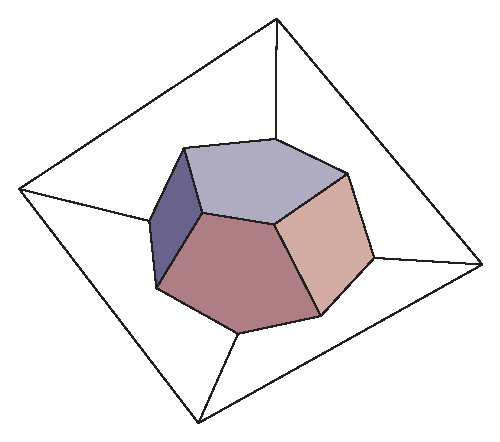
\includegraphics{\ps/vor.eps} %% CORRECT GRAPHIC?
  \caption{A truncated Voronoi cell and a subset of the cell lying in a sector}
  \label{voronoi}
\end{figure}

\begin{example} (2D Voronoi cell minimization). Take a packing of disks of
radius $1$ in the plane.  Let $\Lambda$ be the set of centers of
the disks.  Assume that the origin $0\in\Lambda$ is one of the
centers. The truncated Voronoi cell at $0$ is the set of all
$x\in\ring{R}^2$ such that $|x|\le t$, and $x$ is closer to the
origin than to any other center in $\Lambda$.  We assume
$t\in(1,\sqrt2)$.

Only the centers of distance at most $2t$ affect the shape and
area of the truncated Voronoi cell.  For each $n=0,1,2,\ldots$, we
have a topological space of all truncated Voronoi cells with $n$
nonzero disk centers $v_i$ at distance at most $2t$.  Fix $n$, and
let $X$ be the topological space.

Let $D=D_i$, $i=1,\ldots,n$,  be the sectors lying between
consecutive segments $(0,v_i)$.  Each sector is characterized by
its angle $\alpha$ and the lengths $y_a$ and $y_b$ of the two
segments $(0,v_i)$, $(0,v_j)$ between which the sector lies.  The
part $A$ in $D$ of the area of the truncated Voronoi cell is a
function of the variables $\alpha$, $y_a$, $y_b$.  A nonlinear
implicit equation $\phi=0$ relates $A$, $\alpha$, $y_a$, and $y_b$
on $D$. The variables $u_i$ of the linear assembly problem for the
local domain $D$ are $A$, $y_a$, $y_b$, $\alpha$.


We have a linear assembly problem.  The function $c\cdot x$ is the
area of the truncated Voronoi cell, viewed as a sum of variables
$A$, for each sector $D$ (or rather, their pullbacks to $X$ under
the natural projections $X\to D$).

The assembly constraints are all linear. One linear relation
imposes that the angles of the $n$ different sectors must sum to
$2\pi$. Other linear relations impose that the variable $y_a$ on
$D$ equals the variable $y_b$ on $D'$ if the two variables
represent the length of the same segment $(0,v_i)$ in $X$.
\end{example}


\subsection{solving linear assembly problems}

In this section we describe how various linear assembly problems
are solved in the proof of the Kepler conjecture in terms
sufficiently general to apply to other linear assembly problems as
well.

Let us introduce some general notation.  Let $x_D = (x_i:
\op{dom}(u_i)=D)$ be the vector of variables with local domain
$D$. Write $c\cdot x$ in the form $\sum_D c_D\cdot x_D$ and the
assembly conditions as
$$A \,x =\sum_D A_D x_D,$$
according to the local domain of the variable.


\subsubsection{Linear relaxation}
The first general technique is {\it linear relaxation}. We replace
the nonlinear relations $\phi(x_D)\ge0, \phi\in\Phi_D$ with a
collection of linear inequalities that are true whenever the
constraints $\Phi_D$ are satisfied: $A'_D x_D \le b_D$.  A linear
program is obtained by replacing the nonlinear constraints
$\Phi_D$ with the linear constraints. Its solution dominates the
nonlinear optimization problem.  In this way, the nonlinear
maximization problem can be bounded from above.

Let us review some constructions that insure rigor in linear
programming solutions. We assume general familiarity with the
basic theory and terminology of linear programming. It is
well-known that the primal has a feasible solution iff the dual is
bounded.  We will formulate our linear programs in such a way that
both the primal and the dual problems are feasible and bounded.

We use vector notation to formulate a primal problem as
    \begin{equation}
        \max\, c\cdot x
        \label{cx}
    \end{equation}
such that $A x \le b$, where $x$ is a column vector of free
variables (no positivity constraints), $A$ is a matrix, $c$ is a
row vector, and $b$ is a column vector.

We can insure that this primal problem is bounded by bounding each
of the variables $x_i$.  (This is easily achieved considering the
geometric origins of our problem, which provides interpretations
of variables as particular dihedral angles, edge lengths, and
volumes.) We assume that these bounds form part of the constraints
$A x\le b$.

The linear programs we consider have the property that if the
maximum is less than a constant $K$, the solution does not
interest us.  (For instance, in the dodecahedral conjecture,
Voronoi cell volumes are of interest only if the volume is less
than the volume of the regular dodecahedron.) This observation
allows us to replace the primal problem with one having an
additional variable $t$:
    %%


\subsection{nonlinear duality}
The second general technique is nonlinear duality.  Suppose that
we wish to show that the maximum of the primal problem~\ref{cx} is
at most $M$.

Let $x^* = (x^*_D)$ be a guess of the solution to the problem,
obtained for example, by numerical nonlinear optimization. We
relax the nonlinear optimization by dropping from the matrix $A$
and the vector $b$ those inequalities that are not binding at
$x^*$. With this modification, we may assume that $A\,x^*=b$.  Let
$m$ be the size of the vector $b$, that is, the number of binding
linear conditions. Let $d$ be the number of local domains $D$.

We introduce a linear dual problem with real variables $t$,
$r_\phi: \phi\in\Phi_D$, and $w\in\ring{R}^m$. The variables
$r_\phi$ and $w$ are constrained to be non-negative.

We consider the linear problem of maximizing $t$ such that
    \begin{equation}
        M + d\, t - c\cdot x^* \ge 0
        \label{Mx}
    \end{equation}
and such that for each $x_D$ in each $D$ the linear inequality
    \begin{equation}
        c_D\cdot (x_D-x^*_D) + \sum_{\Phi_D} r_\phi \phi(x) +
                    w A_D (x^*_D-x_D) + t
            < 0
        \label{xD}
    \end{equation}
is satisfied.

There is no guarantee that a feasible solution exists to this
system of inequalities.  However, any feasible solution gives an
upper bound $M$. Indeed, let $x=(x_D)$ be any feasible argument to
the primal, and let $t,r_\phi,w$ be a feasible solution to the
dual. Taking the sum of the linear inequalities~\ref{xD}, over $D$
at $x$, we have (recall $\phi\ge0$ and $A x\le b$):
$$
\begin{array}{lll}
M &\ge M + c\cdot (x-x^*) + \sum_D\sum_{\Phi_D} r_\phi \phi(x)
    + w A (x^*-x) + d\, t,\\
    &\ge c\cdot x + (M + d\, t - c\cdot x^*) + w (b-A x),\\
    &\ge c\cdot x.
\end{array}
$$

Since the dual problem has infinitely many constraints (because of
constraints for each $x\in D$), we solve the dual problem in two
stages. First, we approximate each $D$ by a finite set of test
points, and solve the finitely constrained linear programming
problem for $t, r_\phi$, and $w$.

We replace $t$ with $t_0 = (-M +c\cdot x^*)/d$ (to make the
constraint \ref{Mx} bind).  It follows from the feasibility of $t$
that $t\ge t_0$, and that $t_0,r_\phi,w$ is also feasible on the
finitely constrained problem. To show that $t_0,r_\phi,w$
satisfies all the inequalities~\ref{xD} (under the substitution
$t\mapsto t_0$), we use interval arithmetic to show that each of
these inequalities hold. (To make these interval arithmetic
verifications as easy as possible, we have chosen the solution
$t_0,r,w$ to make the closest inequality hold by as large a margin
$t-t_0$ as possible. This is the meaning of the maximization over
$t$ in the dual problem.)  The next section will give further
details about interval arithmetic verifications.

\subsection{branch and bound}
The third technique is branch and bound.  When no feasible
solution is found in step (2), it may still be possible to
partition $X$ into finitely many sets $X = \coprod X_i$, on which
feasible solutions to the dual may be found.  Although this is an
essential part of the solution, the rules for branching in the
Kepler conjecture follow the structure of that problem, and we do
not give a general branching algorithm.


\section{Definitions and Interpretations}

\begin{definition}
By $\optt{quarter}(\alpha)$ we mean that at dart $\alpha$, we have
an upright quarter.
\end{definition}

\begin{definition}
By $\optt{ancsim}(\alpha)$ we mean that at dart $\alpha$ we have an upright
diagonal and an anchored simplex: $\optt{azim}\slt \pi$ and
the opposite edge length is at most $3.2$ and at least $2$.
\end{definition}

\begin{definition}
By $\optt{gap}(\alpha)$ we mean that at dart $\alpha$, we have an
upright diagonal $\optt{azim}\slt \pi$ and the opposite edge length
is greater than $3.2$.
\end{definition}

\begin{definition}
By $\optt{upright}(\alpha)$ we mean that at $\alpha$ there is an upright
diagonal.
\end{definition}

\section{Listing of Assembly Problems}


\begin{lemma}\dcg{Sec~11.7}{118}  Let $H=(D,n,e,f)$ be a geometric
hypermap.  Let $N$ 
be a node of $H$ of cardinality 5.    Assume that for all $\alpha\in N$
  $$
  \optt{upright}(\alpha).
  $$
Then $\optt{azim}(\alpha)\slt \pi$ for all $\alpha\in N$.
Hence $\optt{gap}(\alpha)$ or $\optt{ancsim}(\alpha)$.
\end{lemma}

\begin{lemma}\dcg{Sec~11.7,Rem~11.3}{118}  Let $H$ be a geometric
hypermap.  Let $N$ 
be a node of $H$ of cardinality 5.   Assume that $\optt{upright}(\alpha)$
for $\alpha\in N$.  There is a set $S\subset N$ of cardinality at most
$2$ such that $\optt{gap}(\alpha) \Rightarrow \alpha\in S$.
\end{lemma}

\begin{lemma}\dcg{Lemma~11.14}{119}  Let $H$ be a geometric
hypermap.  Let $N$ be a node of $H$ of cardinality $5$.  Assume
that $\optt{upright}(\alpha)$ for $\alpha\in N$.  Assume that there
is a set $S\subset N$ of cardinality $3$ such that
  $$\optt{quarter}(\alpha)\Leftrightarrow \alpha\in S.$$
Then 
  $$
  \sum_{\alpha\in S} \optt{tau\_nu}(\alpha) \sgt \squander.
  $$
\end{lemma}